% Beamer do material do curso de Verão (2015) do IME-USP
% Introdução ao Projeto de Jogos
%
% Baseado no template LaTeX das apresentações do LIDET versão 2
% (https://github.com/luigivieira/LIDET)
%

\providecommand\classopts{}
\expandafter\documentclass\expandafter[table, usenames, svgnames, dvipsnames, \classopts]{beamer}

\usepackage{etex}
\usepackage{beamerthemeshadow}
\usepackage[portuguese]{babel}
\usepackage[utf8]{inputenc}
\usepackage[absolute,overlay]{textpos}
\usepackage{array}
\usepackage{framed}
\usepackage{booktabs}
\usepackage[compatibility=false]{caption}
\usepackage{subcaption}
\usepackage{outlines}
\usepackage{ulem}
\usepackage{xcolor,colortbl}
\usepackage{ragged2e}
\usepackage{tikz}

% ---------------------------------------------------------------------------- %
% Presentation definitions
% ---------------------------------------------------------------------------- %
\usetheme{Luebeck}
\hypersetup{pdfpagemode=FullScreen} % Starts the presentation in full screen

% layout
\setbeamerfont{frametitle}{size=\normalsize}
\setbeamerfont{title}{size=\normalsize}
\beamertemplatenavigationsymbolsempty
\setbeamertemplate{bibliography item}[text]%
\setbeamertemplate{headline}{} % Remove upper bar

% colors
\definecolor{lidet_orange}{rgb}{0.9, 0.49, 0.09}
\definecolor{lidet_black}{rgb}{0.2, 0.2, 0.2}

\setbeamercolor{title}{bg=lidet_orange}
\setbeamercolor{structure}{bg=white, fg=lidet_orange}
\setbeamercolor{normal text}{fg=black}
\setbeamercolor{section in head/foot}{fg=white, bg=lidet_black}
\setbeamercolor{postit}{fg=white, bg=lidet_orange!90!lidet_black}

% shadow
\makeatletter
\pgfdeclareverticalshading[black,bg]{bmb@shadow}{200cm}{%
  color(0bp)=(lidet_black!25); color(4bp)=(black!50!bg); color(8bp)=(black!50!bg)}
\pgfdeclareradialshading[black,bg]{bmb@shadowball}{\pgfpointorigin}{%
  color(0bp)=(black!50!bg); color(4bp)=(lidet_black!25)}
\pgfdeclareradialshading[black,bg]{bmb@shadowballlarge}{\pgfpointorigin}{%
  color(0bp)=(black!50!bg); color(4bp)=(black!50!bg); color(8bp)=(lidet_black!25)}
%
\makeatother

% Captions for images and tables
\setlength{\abovecaptionskip}{5pt plus 5pt minus 5pt}
\setlength{\belowcaptionskip}{5pt plus 5pt minus 5pt}
\captionsetup[figure]{font=scriptsize,labelfont=scriptsize}
\captionsetup[table]{font=scriptsize,labelfont=scriptsize}
\captionsetup{labelformat=empty,labelsep=none}

% Dimensions for table rules
\setlength\heavyrulewidth{0.1em} 
\setlength\lightrulewidth{0.01em}
\setlength\belowrulesep{0.10ex}
\setlength\aboverulesep{0.10ex}

% Define macros to mark the begining and ending of references
% Basically, handles the automatically spanned frames (due to parameter allowframebreaks)
% as backup frames, so they do not influence in the frame numbering
\newcommand{\referencesbegin}{
   \newcounter{framenumberappendix}
   \setcounter{framenumberappendix}{\value{framenumber}}
}
\newcommand{\referencesend}{
   \addtocounter{framenumberappendix}{-\value{framenumber}}
   \addtocounter{framenumber}{\value{framenumberappendix}} 
}

% Adjust footnotes to not overlap the footbar
\addtobeamertemplate{footnote}{}{\vspace{1.0ex}}
\let\oldfootnotesize\footnotesize
\renewcommand*{\footnotesize}{\oldfootnotesize\tiny}

% Redefine the quote environment so short quotes are not broken easily
\renewenvironment{quote}
	{\list{}{\leftmargin1em\rightmargin\leftmargin}%
	\item\relax}
	{\endlist}

% Section frames (that appear before each section)
\AtBeginSection[] 
{
	{
		\setbeamertemplate{footline}{} % Hide the footline locally for these frames
		\begin{frame}<beamer>[noframenumbering]
			\begin{center}
				\begin{tikzpicture}
					\node[align=left, left color=lidet_orange, right color=lidet_orange, draw, rounded corners, minimum width=10cm, minimum height=1cm] {\color{white} \textbf{\insertsectionhead}};
				\end{tikzpicture}
			\end{center}
			\footnotesize{ \tableofcontents[currentsection, hideothersubsections] }
		\end{frame}
	}
}

\AtBeginSubsection[]
{
    \begin{frame}
        \centering
        \Large
        \textbf{\insertsubsection}
    \end{frame}
}

\AtBeginSubsubsection[]
{
    \begin{frame}
        \centering
        \large
        \insertsubsection
        \vskip 1em
        \Large
        \textbf{\insertsubsubsection}
    \end{frame}
}

\DeclareGraphicsExtensions{.pdf,.jpg,.png}
\graphicspath{{./images/}}

% ---------------------------------------------------------------------------- %
% Presentation title, author and institution
% ---------------------------------------------------------------------------- %
\newcommand{\lessontitle}{Aula 1 - Enxergando Jogos como Sistemas}
\title{\textbf{Introdução ao Projeto de Jogos}}
\subtitle{{\small \lessontitle}}

\newcommand{\autores}{Luiz C. Vieira, Vinícius K. Daros}
\author[\autores]{\scriptsize
    Luiz Carlos Vieira e Vinícius Kiwi Daros\\
    \{luigivieira,vinicius.k.daros\}@gmail.com
}

\newcommand{\lidet}{LIDET (IME - USP)}
\institute[\lidet]{\\[1.0mm]
Curso de Verão (2015)\\
Departamento de Ciência da Computação}

\date{{\tiny 12 de Janeiro de 2015}}

% ---------------------------------------------------------------------------- %
% Presentation content
% ---------------------------------------------------------------------------- %

% ---------------------------------------------------------------------------- %
\begin{document}
% ---------------------------------------------------------------------------- %

% ---------------------------------------------------------------------------- %
% First Slide (index 0) = cover
% ---------------------------------------------------------------------------- %

{%\usebackgroundtemplate{}} 
\begin{frame}[plain, noframenumbering]

	\begin{columns}[c]
		\column{0.2\textwidth}
			\hspace*{-1.5em}
			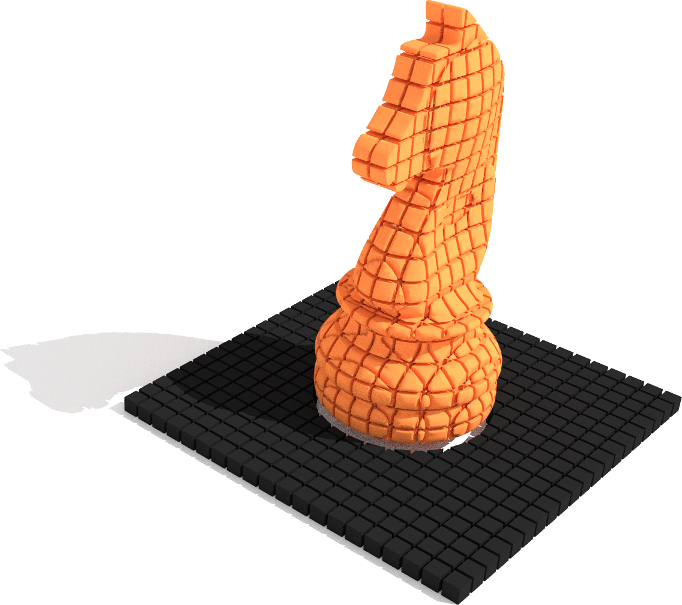
\includegraphics[width=0.35\paperwidth]{side_bar}\\
		\column{0.01\textwidth}
		\column{0.70\textwidth}
			\titlepage
			\hspace*{+0.5em}
			\begin{center}
				
\includegraphics[height=1.0cm]{lidet-logo}\\
				
\includegraphics[height=1.0cm]{ime-logo}\\
			\end{center}
	\end{columns}
	%\addtocounter{framenumber}{-1}
\end{frame}
}

% ---------------------------------------------------------------------------- %
% Other Slides (index from 1 onwards)
% ---------------------------------------------------------------------------- %

% setup navigation symbols and footline
\setbeamertemplate{navigation symbols}{}
\makeatletter
\setbeamertemplate{footline}{%
    \leavevmode%
    \hbox{%
        \begin{beamercolorbox}[wd=0.28\paperwidth,ht=4ex,dp=1ex,left,%
                               leftskip=2ex]{author in head/foot}%
            \usebeamerfont{title in head/foot}
            \insertdate\newline%
            \vskip 0.6ex%
            \autores
        \end{beamercolorbox}%
        \begin{beamercolorbox}[wd=0.53\paperwidth,ht=4ex,dp=1ex,center]%
                              {author in head/foot}%
            \usebeamerfont{author in head/foot}\lessontitle%
        \end{beamercolorbox}%
        \begin{beamercolorbox}[wd=0.19\paperwidth,ht=4ex,dp=1ex,right,%
                               rightskip=2ex]{author in head/foot}%
            \insertframenumber{}/\inserttotalframenumber \newline
            \lidet%
        \end{beamercolorbox}%
    }%
    \vskip 4cm%
}
\makeatother

% ---------------------------------------------------------------------------- %
\begin{frame}[plain]
\frametitle{\textbf{Agenda}}

	\hspace*{+4.0em}
	\footnotesize{ \tableofcontents }
\end{frame}

% ---------------------------------------------------------------------------- %
\section{Introdução}
% ---------------------------------------------------------------------------- %

\subsection{Provimento e motivação}

% ------------------------------
\begin{frame}
	\frametitle{\textbf{Laboratório}}
	
	\begin{center}
		
\includegraphics[height=0.2\paperheight]{lidet-logo}\\
		\url{http://www.ime.usp.br/~lidet}
	\end{center}
	
	\vspace{2em}
	
	\begin{outline}
		\1 Criado e gerido pelo Prof. Dr. Flávio Soares Corrêa da Silva
			\2[-] {\scriptsize origem no LIAMF (Laboratório de Inteligência Artificial e Métodos Formais)}
			\2[-] {\scriptsize dentro do Departamento de Ciência da Computação do IME-USP}
		
		\vspace{1em}
		
		\1 Pesquisas em interatividade e entretenimento digital
			\2[-] {\scriptsize governo eletrônico, interoperabilidade entre museus, inteligência artificial em jogos eletrônicos, avaliação de experiência de jogadores}
	\end{outline}	

\end{frame}

% ------------------------------
\begin{frame}
	\frametitle{\textbf{Ministrantes}}
	
	\begin{columns}[c]
	
		\column{0.2\textwidth}
		
			\begin{center}
				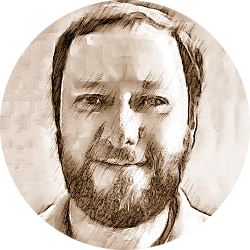
\includegraphics[height=0.2\paperheight]{luiz}\\
				\textbf{Luiz \mbox{Carlos Vieira}}
			\end{center}
			
		\column{0.8\textwidth}
		
			\begin{outline}
				\1 Doutorando em Ciência da Computação
					\2[-] {\scriptsize avaliação de diversão em jogos digitais por meio do rastreamento e análise de expressões faciais}
				
				\vspace{1em}
				
				\1 Projetista de jogos de tabuleiro
					\2[-] {\scriptsize coautor de Turned (publicado na Europa), Xôôô Peste e Reviravolta (em publicação)}
			\end{outline}
			
	\end{columns}		
		
	\vspace{2em}
		
	\begin{columns}[c]		

		\column{0.8\textwidth}
			
			\begin{outline}
				\1 Mestrando em Ciência da Computação
					\2[-] {\scriptsize construção de pilotos virtuais com aprendizado de máquina em simuladores automobilísticos}
				
				\vspace{1em}
				
				\1 Integrante do USPGameDev
					\2[-] {\scriptsize grupo de pesquisa e desenvolvimento de jogos digitais e analógicos}
			\end{outline}
		
		\column{0.2\textwidth}
		
			\begin{center}
				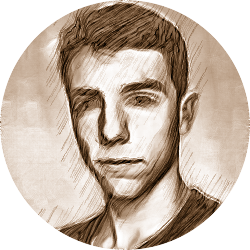
\includegraphics[height=0.2\paperheight]{vinicius}\\
				\textbf{Vinícius Kiwi Daros}
			\end{center}
		
	\end{columns}	

\end{frame}

% ------------------------------
\begin{frame}
	\frametitle{\textbf{Motivação}}
	
	\begin{block}{}
	
		\vspace{1em}
	
		\begin{quotation}
			\noindent
			\justify
			{\large Complementar a formação técnica/operacional de qualidade (leia-se ``Ciência da Computação'') com a capacitação em aspectos humanos relacionados ao \textbf{design de experiências}}
		\end{quotation}

		\vspace{1em}

	\end{block}
	
	\begin{center}
		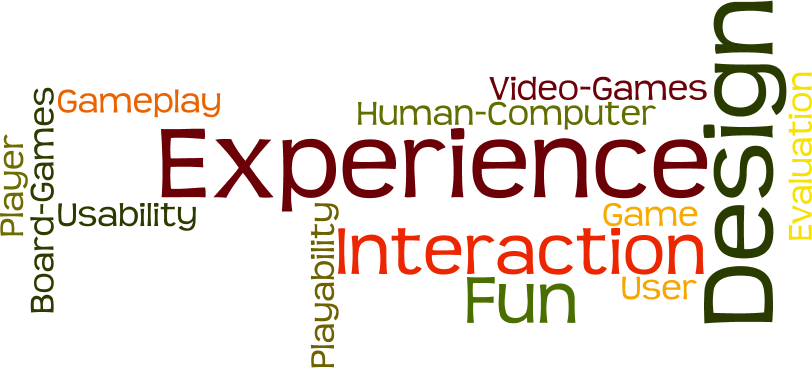
\includegraphics[height=0.4\paperheight]{word-cloud}\\
	\end{center}

\end{frame}

\subsection{Objetivos, programa e bibliografia}

% ------------------------------
\begin{frame} 
	\frametitle{\textbf{Objetivos}}
	
	\begin{outline}[enumerate]
		\1 Introduzir os principais conceitos sobre o projeto de jogos (\textit{game design})
			\2[-] {\scriptsize pontualmente destacando as diferentes características dos meios utilizados (digital e analógico/tabuleiro)}
	    
		\vspace{1em}
	    
		\1 Exercitar a construção de um protótipo com fidelidade crescente
			\2[-] {\scriptsize utilizando primordialmente prototipagem em papel}
		
		\vspace{1em}
			    
		\1 Exercitar a avaliação da experiência de jogo (\textit{playtesting})
			\2[-] {\scriptsize executando e analisando avaliações heurísticas e sessões de jogo com jogadores planejados e reais}
	\end{outline}
	
\end{frame}

% ------------------------------
\begin{frame} 
	\frametitle{\textbf{Programa}}
	
	\begin{columns}[c]
		
		\column{0.2\textwidth}

		\column{0.8\textwidth}
	
			\begin{outline}
			
				\1[\textbf{12/01 (segunda)}:] Enxergando jogos como sistemas
					\2[-] {\scriptsize jogos sob a ótica do designer}
					\2[-] {\scriptsize desconstrução de jogos clássicos}
			    
				\vspace{0.5em}
			    
				\1[\textbf{13/01 (terça)}:] Pensando nas regras do jogo
					\2[-] {\scriptsize comunicação, documentação e público-alvo}
					\2[-] {\scriptsize detalhamento da mecânica}
				
				\vspace{0.5em}
					    
				\1[\textbf{14/01 (quarta)}:] Pensando na experiência de jogo
					\2[-] {\scriptsize experiência pragmática (jogabilidade x \textit{gameplay})}
					\2[-] {\scriptsize interatividade e interação (CCC)}
		
				\vspace{0.5em}
					    
				\1[\textbf{15/01 (quinta)}:] Pensando na estética do jogo
					\2[-] {\scriptsize experiência hedônica (\textit{juiceness})}
					\2[-] {\scriptsize contorno e exploração de problemas}
		
				\vspace{0.5em}
					    
				\1[\textbf{16/01 (sexta)}:] Realizando avaliações e testes (\textit{playtesting})
					\2[-] {\scriptsize avaliação heurística}
					\2[-] {\scriptsize \textit{playtesting} com participantes}
					
			\end{outline}	

	\end{columns}

	\hfill

\end{frame}

% ------------------------------
\begin{frame} 
	\frametitle{\textbf{Avisos importantes}}
	
	\begin{block}{\centering\textbf{ATENÇÃO!}}
	
		\begin{outline}
			\1 As aulas ocorrem pela manhã, no período entre 09:00 e 12:00
				\2[-] {\scriptsize \textbf{não se atrase!}}
				\2[-] {\scriptsize as aulas começam no horário programado}
		    
			\vspace{1em}
		    
			\1 Apesar de bastante conteúdo expositivo, as aulas são primordialmente práticas
				\2[-] {\scriptsize \textbf{traga seu próprio material!}}
				\2[-] {\scriptsize  para documentação e construção de protótipos:\\ \textit{caderno, sulfites, régua, tesoura, cola, fita adesiva, lápis, borracha, canetas coloridas, cartolina, dados, cartas de baralho, botões, feijões, ...}}
			
			\vspace{1em}
				    
			\1 O curso se encerra com a execução de avaliações do protótipo criado em aula
				\2 {\scriptsize \textbf{não esqueça o projeto/material em casa!}}
				\2 {\scriptsize infelizmente não há espaço para armazená-lo na USP}
		\end{outline}

	\end{block}	
	
\end{frame}

% ------------------------------
\begin{frame} 
	\frametitle{\textbf{Bibliografia básica}}
	
	\begin{columns}[c]
	
		\column{0.33\textwidth}
			\begin{center}
				\frame{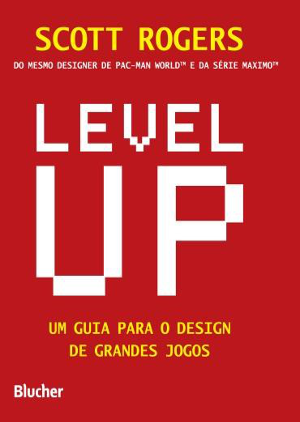
\includegraphics[height=0.5\paperheight]{rogers}}\\
				Scott Rogers\\[0.5em]
				\textit{{\large Level UP: Um Guia para o Design de Grandes Jogos}}\\[0.5em]
				{\small Blucher, 2013}
			\end{center}
			
		\column{0.33\textwidth}
			\begin{center}
				\frame{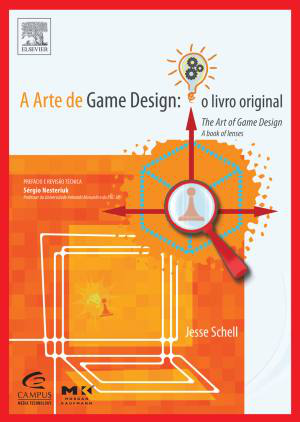
\includegraphics[height=0.5\paperheight]{schell}}\\
				Jesse Schell\\[0.5em]
				\textit{{\large A Arte De Game Design: O Livro Original}}\\[0.5em]
				{\small Elsevier, 2010}
			\end{center}
			
		\column{0.33\textwidth}
			\begin{center}
				\frame{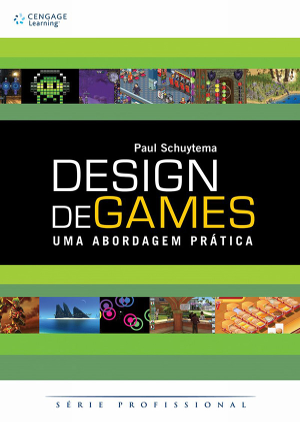
\includegraphics[height=0.5\paperheight]{schuytema}}\\
				Paul Schuytema\\[0.5em]
				\textit{{\large Game Design: Uma Abordagem Prática - Série Profissional}}\\[0.5em]
				{\small Cengage Learning, 2008}
			\end{center}
			
	\end{columns}
	
\end{frame}

% ------------------------------
\begin{frame} 
	\frametitle{\textbf{Material do curso}}
	
	\begin{center}
		{\large
			As apresentações\footnote{Sem as imagens com copyright} do curso estarão disponíveis em:\\[1em]
			\url{http://www.ime.usp.br/~lidet/projeto-jogos/}
		}
	\end{center}
	
\end{frame}

% ---------------------------------------------------------------------------- %
\section{O Design de Jogos}
% ---------------------------------------------------------------------------- %

\subsection{Conceitualização}

% ------------------------------
\begin{frame}
	\frametitle{\textbf{O que é um jogo?}}

	\begin{center}
		A atividade dessas crianças é um jogo ou uma brincadeira?
	\end{center}	

	\vspace{-2em}
	
	\begin{figure}
		\centering
		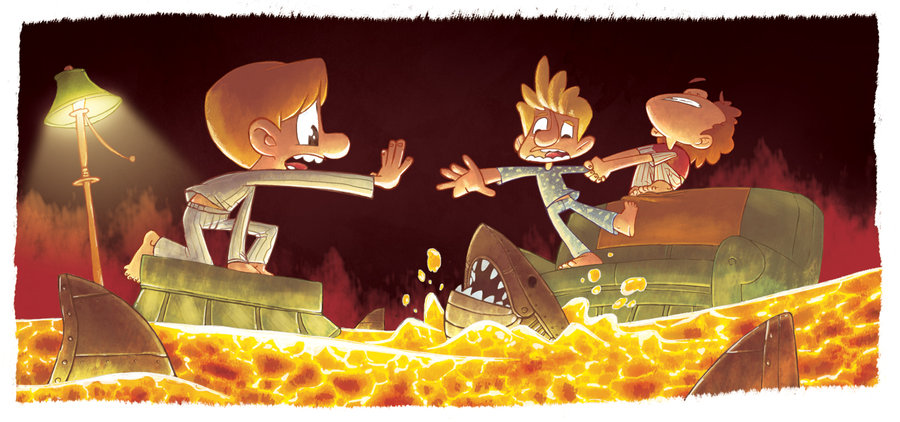
\includegraphics[width=0.9\paperwidth]{floor-is-lava}
		\caption{\textbf{The Floor is Lava} \copyright{2011-2015} DerekHunter\footnote{\url{http://derekhunter.deviantart.com/art/The-Floor-is-Lava-276153571}}}
	\end{figure}
	
	\vspace{2em}

\end{frame}

% ------------------------------
\begin{frame}
	\frametitle{\textbf{O que torna atividades lúdicas divertidas}}

	As atividades lúdicas envolvem aprendizado em três dimensões \cite{Malone1980}:

	\vspace{1em}

	\begin{outline}
		\1 Curiosidade
			\2[-] {\scriptsize comportamento exploratório decorrente do interesse natural em adquirir conhecimento}
			
		\vspace{1em}
		
		\1 Desafio
			\2[-] {\scriptsize oportunidades para ação em que há um balenceamento entre dificuldade e habilidade}
					
		\vspace{1em}
		
		\1 Fantasia
			\2[-] {\scriptsize imagens mentais não presentes nos sentidos que ajudam a acomodar a realidade}
	\end{outline}
\end{frame}

% ------------------------------
\begin{frame}
	\frametitle{\textbf{A teoria do fluxo}}

	\begin{figure}
	    \centering
        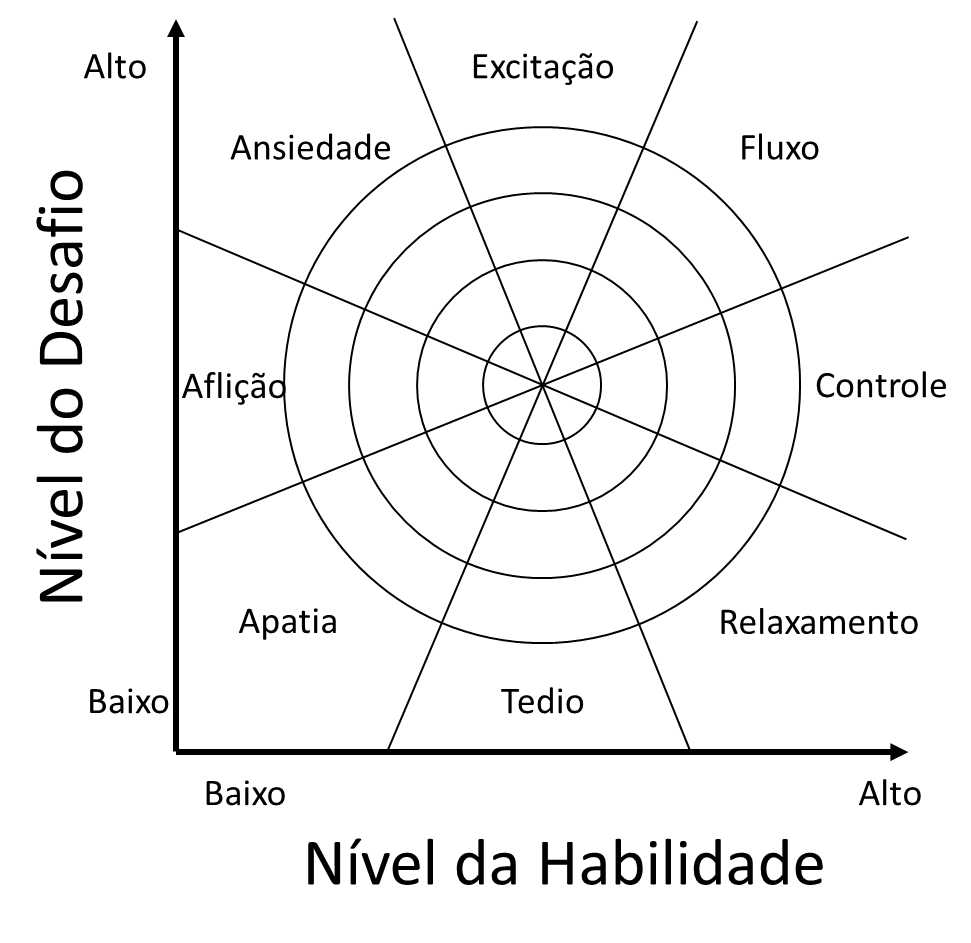
\includegraphics[height=0.8\paperheight]{flow-model}
        \caption{\textbf{Modelo dos estados do Fluxo}, baseado em \cite{Nakamura2001}}
    \end{figure}

\end{frame}

% ------------------------------
\begin{frame}
	\frametitle{\textbf{Diferentes tipos de experiências}}

	\begin{table}
		\tiny
		\setlength{\tabcolsep}{5pt}
		\renewcommand{\arraystretch}{1}
		\caption{\textbf{A dinâmica da experiência em interações individuais e sociais}, baseado em \cite{Forlizzi2004}}
		\begin{tabular}{ll}
			\toprule
			\textbf{Tipo de Interação} & \textbf{Descrição}\\
			\midrule
			Fluente & Automática e bem aprendida, não compete por atenção\\
			Cognitiva & Requer esforço atentivo e resulta em conhecimento ou confusão\\
			Expressiva & Auxilia na formação de relacionamento com o produto/atividade\\
			\bottomrule
		\end{tabular}
	\end{table}

	\vspace{-1em}

 	\begin{figure}
	    \centering
        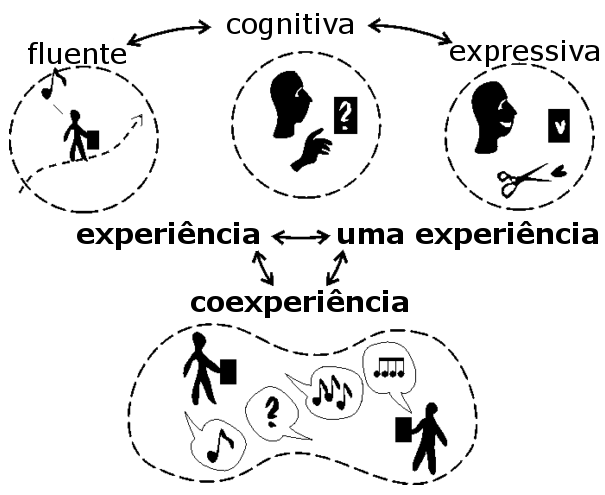
\includegraphics[height=0.5\paperheight]{experience-dynamics}
    \end{figure}
    
	\vspace{-1em}
	    
	\begin{table}
		\tiny
		\setlength{\tabcolsep}{5pt}
		\renewcommand{\arraystretch}{1}
		\begin{tabular}{ll}
			\toprule
			\textbf{Tipo de Experiência} & \textbf{Descrição}\\
			\midrule
			Experiência & Fluxo constante de interação com o produto/atividade\\
			Uma experiência & Pode ser articulada e inspira mudanças comportamentais e emocionais\\
			Coexperiência & Cria significado e emoção a partir do uso conjunto\\
			\bottomrule
		\end{tabular}
	\end{table}

\end{frame}

% ------------------------------
\begin{frame}
	\frametitle{\textbf{Diversão, jogar e brincar}}

	Segundo Jesse Schell:

	\vspace{1em}

	\begin{outline}
		\1 Diversão é o prazer com surpresas
	    
		\vspace{1em}
	    
		\1 Jogar e brincar (\textit{play}) são manipulações que saciam a curiosidade
		
		\vspace{1em}
			    
		\1 Um brinquedo é um objeto com o qual se brinca

		\vspace{1em}
			    
		\1 Um bom brinquedo é um objeto com o qual é divertido brincar

		\vspace{1em}
			    
		\1 Um jogo é uma atividade de resolução de problemas, encarada com uma atitude lúdica
			
	\end{outline}

\end{frame}

% ------------------------------
\begin{frame} 
	\frametitle{\textbf{Tipos de atividades lúdicas}}

	O nível de interatividade de uma atividade lúdica permite uma classificação hierárquica:
	
    \begin{figure}
	    \centering
   		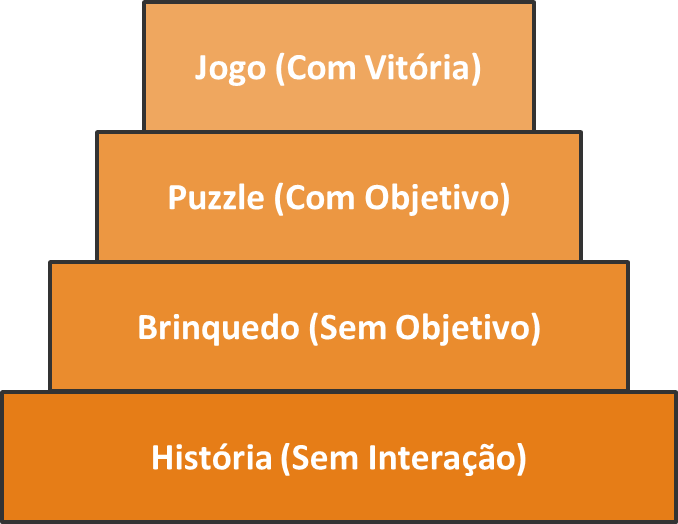
\includegraphics[height=0.5\paperheight]{types-of-play}
        \caption{\textbf{Hierarquia das atividades lúdicas}, baseado em \cite{Fullerton2008}}
    \end{figure}

\end{frame}

% ------------------------------
\begin{frame} 
	\frametitle{\textbf{Tipos de atividades lúdicas}}

	Um eixo adicional relacionado à forma projetada fornece uma classificação mais elaborada de produtos/atividades interativos:
	
    \begin{figure}
	    \centering
        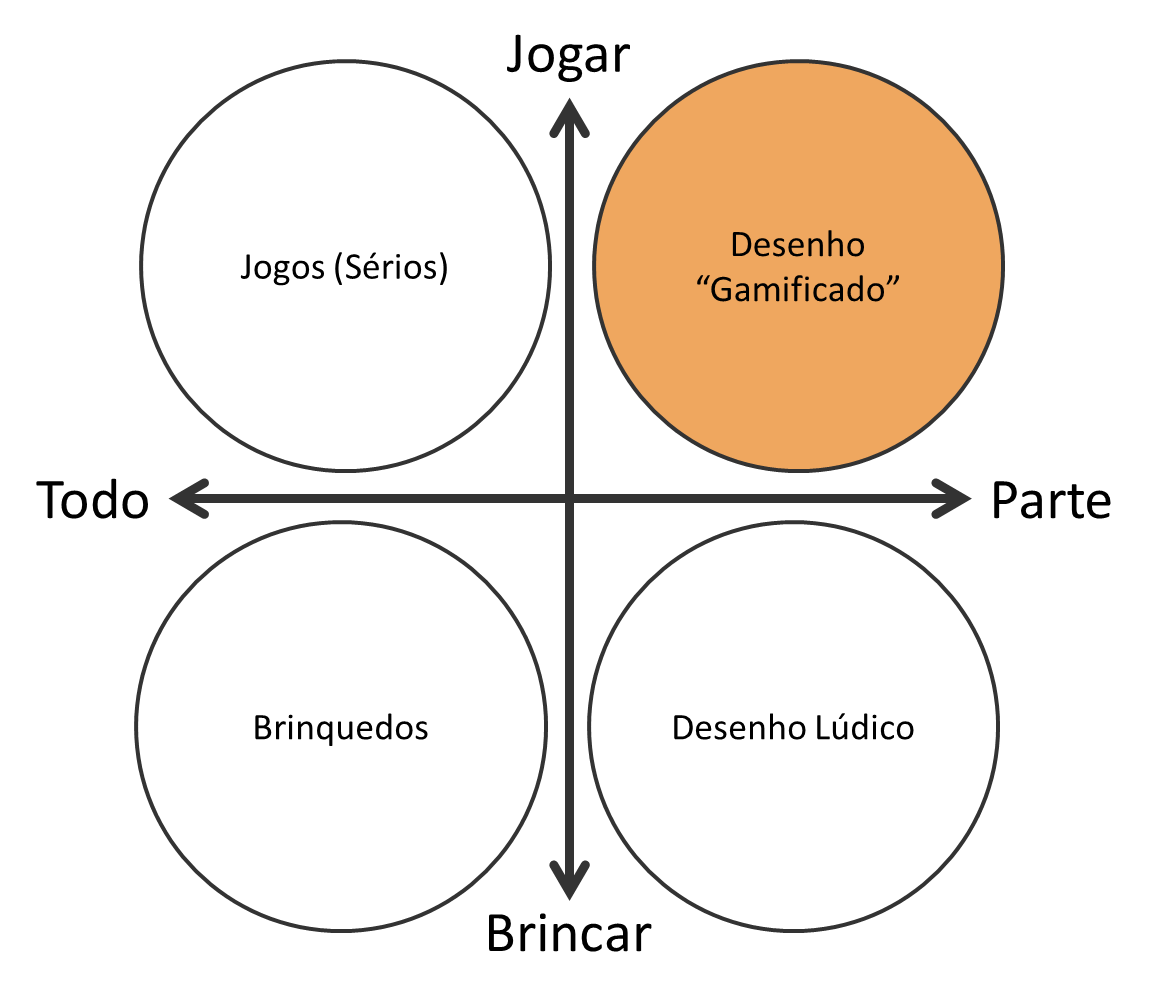
\includegraphics[height=0.65\paperheight]{taxonomy}
        \caption{\textbf{Taxonomia das atividades lúdicas com os eixos jogar-brincar e todo-parte}, baseado em \cite{Groh2012}}
    \end{figure}

\end{frame}


\subsection{O que são jogos}

% ------------------------------
\begin{frame}
	\frametitle{\textbf{O que é um jogo?}}
	
	Eis \emph{uma} definição possível \cite{Fullerton2008}:

	\vspace{0.2em}
	
	\begin{outline}
		\1 Um sistema fechado e \emph{formal} (isto é, com regras)
		
		\vspace{0.5em}
		
		\1 Que engaja jogadores em \emph{conflitos} estruturados

		\vspace{0.5em}
		
		\1 E resolve as \emph{incertezas} com resultados desiguais
	\end{outline}	

	\vspace{1.5em}

	Tal definição advém do mecanismo psicológico da atenção \cite{Koster2004}:

	\vspace{0.2em}

	\begin{outline}
		\1 Conflitos não são apenas desafios e competição
			\2[-] {\scriptsize são principalmente aspectos interessantes (curiosos)}
		
		\vspace{1em}
		
		\1 Incertezas são padrões familiares ainda parcialmente compreendidos
			\2[-] {\scriptsize jogos fornecem tais padrões para os jogadores ``digerirem'' (\textit{chunking})}
	\end{outline}

\end{frame}

% ------------------------------
\begin{frame}
	\frametitle{\textbf{Qual é o papel do projetista?}}

	O jogo é também um meio de comunicação entre projetista (\textit{game designer}) e jogador (\textit{player})

	\vspace{1em}

	\begin{outline}
		\1 O projetista toma decisões baseadas em melhores práticas
			\2[-] {\scriptsize intencionando elicitar certas experiências nos jogadores}
		
		\vspace{1em}
		
		\1 O jogador tem uma experiência única
			\2[-] {\scriptsize decorrente de histórico e preferências individuais}
			\2[-] {\scriptsize e também do contexto de uso do produto}
	\end{outline}
	
 	\begin{figure}
	    \centering
        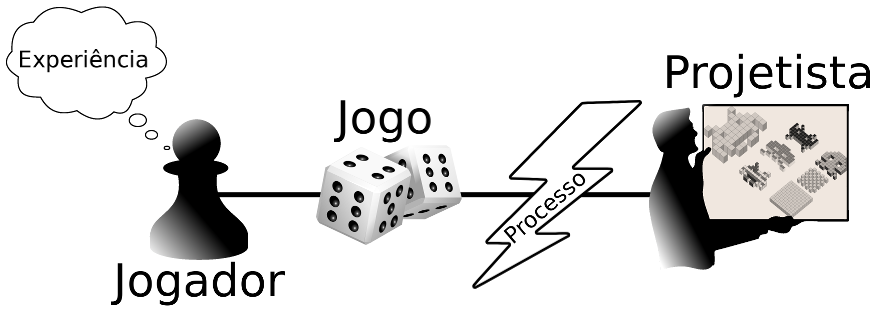
\includegraphics[height=0.3\paperheight]{processo-experiencia}
        \caption{\textbf{Agentes envolvidos no processo de criação de jogos}, baseado nas ilustrações de Jesse Schell}
    \end{figure}

\end{frame}

\subsection{Estrutura de jogos}

% ------------------------------
\begin{frame}
	\frametitle{\textbf{Elementos básicos de um jogo}}

	\begin{columns}[c]
	
		\column{0.45\textwidth}
		
		    \vspace{-2em}
		
			\begin{figure}
			    \centering
		        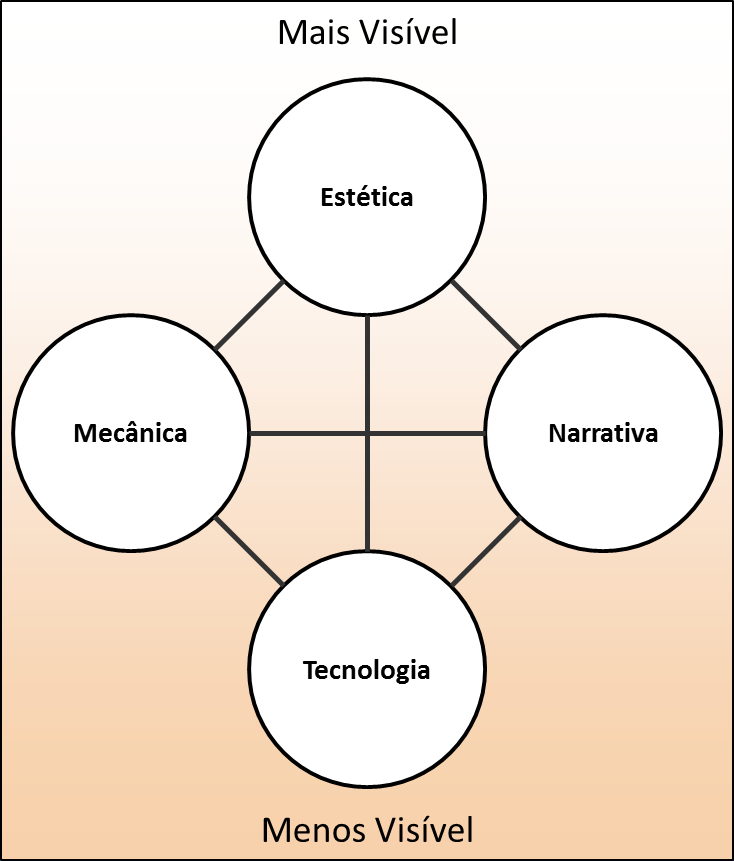
\includegraphics[height=0.65\paperheight]{game-elements}
		        \vspace{0.5em}
		        \caption{\textbf{O tetraedro elemental dos jogos}, baseado na ilustração original de Jesse Schell}
		    \end{figure}
		    
		\column{0.55\textwidth}
		
		    \vspace{-1em}
		
			\begin{outline}
				\1 Mecânica
					\2[-] {\scriptsize procedimentos e regras do jogo}
					\2[-] {\scriptsize descreve objetivo e ações possíveis}

				\vspace{0.5em}

				\1 Estética
					\2[-] {\scriptsize aparência e sentimento do jogo}
					\2[-] {\scriptsize impacto mais direto na experiência do jogador}
				
				\vspace{0.5em}
					
				\1 Narrativa
					\2[-] {\scriptsize sequência de eventos no jogo}
					\2[-] {\scriptsize linear, pré-configurada ou emergente}

				\vspace{0.5em}

				\1 Tecnologia
					\2[-] {\scriptsize materiais e interações que tornam o jogo possível}
					\2[-] {\scriptsize papel, computadores, \textit{lasers}, etc}
			\end{outline}
		
	\end{columns}

\end{frame}

% ------------------------------
\begin{frame}
	\frametitle{\textbf{Jogos e outras formas de entretenimento}}

	\begin{outline}
		\1 Livros e filmes envolvem tecnologia, narrativa e estética
		
		\vspace{0.5em}
		
		\1 Mas não envolvem mecânica!
	\end{outline}

	\vspace{2em}

	\begin{block}{}
	
		\vspace{1em}
	
		\begin{center}
			{\Large A mecânica é o que torna um jogo um jogo}
		\end{center}

		\vspace{0.2em}

	\end{block}

\end{frame}

% ------------------------------
\begin{frame}
	\frametitle{\textbf{Elementos da mecânica}}

	Os seguintes elementos fazem parte da mecânica de qualquer jogo:
	
	\begin{table}
		\scriptsize
		\setlength{\tabcolsep}{5pt}
		\renewcommand{\arraystretch}{1}
		\begin{tabular}{ll}
			\toprule
			\textbf{Objetivo} & \textit{O que o jogador deve alcançar?}\\
			\multicolumn{2}{l}{\hspace{1em} Fornece a oportunidade de encarar desafios e saciar a curiosidade}\\[1em]
			\textbf{Condição de Término} & \textit{Quando o jogo acaba?}\\
			\multicolumn{2}{l}{\hspace{1em} Articula a experiência e estabelece condições de vitória/derrota}\\[1em]
			\textbf{Ações} & \textit{Como o jogador faz para alcançar o objetivo?}\\
			\multicolumn{2}{l}{\hspace{1em} Permitem ao jogador se sentir no controle do ``mundo''}\\[1em]
			\textbf{Feedback} & \textit{Como o jogo ``responde'' ao jogador?}\\
			\multicolumn{2}{l}{\hspace{1em} Fornece o meio para o jogo ``responder'' ao jogador}\\
			\bottomrule
		\end{tabular}
	\end{table}	

	\vspace{-0.5em}

	\begin{block}{}
	
		\vspace{1em}
	
		\begin{center}
			{\large
				Um lembrete importante para quem projeta ``jogos sérios'':\\[1em]
				\emph{O objetivo é do jogador, não do designer!}
			}
		\end{center}

		\vspace{0.2em}

	\end{block}
	
\end{frame}

% ------------------------------
\begin{frame}
	\frametitle{\textbf{Dimensões da estética}}

	\begin{outline}
		\1 Existem diferentes tipos de ``estética'' \cite{Niedenthal2009}
			\2[-] fenômeno sensorial (visual, auditivo, tátil, encorporado)
			\2[-] aspectos apreciativos compartilhados com outras artes
			\2[-] expressão geral da experiência hedônica do jogador
	\end{outline}

	\begin{table}
		\scriptsize
		\setlength{\tabcolsep}{1pt}
		\renewcommand{\arraystretch}{1}
		\caption{\textbf{Estéticas da experiência de jogo} \cite{Hunicke2004}}
		\begin{tabular}{cc}
			\toprule
			\textbf{Sensação} & \textbf{Interação Social}\\
			Jogo como prazer sensorial & Jogo como plataforma social\\[1em]
			\textbf{Fantasia} & \textbf{Descoberta}\\
			Jogo como faz-de-conta & Jogo como território inexplorado\\[1em]
			\textbf{Narrativa} & \textbf{Expressão}\\
			Jogo como drama & Jogo como autodescoberta\\[1em]
			\textbf{Desafio} & \textbf{Submissão}\\
			Jogo como curso de obstáculos & Jogo como passatempo\\
			\bottomrule
		\end{tabular}
	\end{table}
	
\end{frame}

% ------------------------------
\begin{frame}
	\frametitle{\textbf{Jogos digitais x analógicos}}
	
	\begin{quotation}
		\noindent
		{\large Videogames são apenas a evolução natural dos jogos tradicionais em uma nova mídia. As regras que os governam ainda são as mesmas.\\[0.5em]
		\noindent
		\hfill-- Jesse Schell}
	\end{quotation}

\end{frame}

% ------------------------------
\begin{frame}
	\frametitle{\textbf{Desconstrução de jogos}}

	Qualquer jogo existente pode ser ``desconstruído'' nesses elementos:

	\begin{block}{Exemplo: Pong}
	
		\begin{columns}[c]
			
			\column{0.3\textwidth}
			
				\begin{figure}
					\centering
					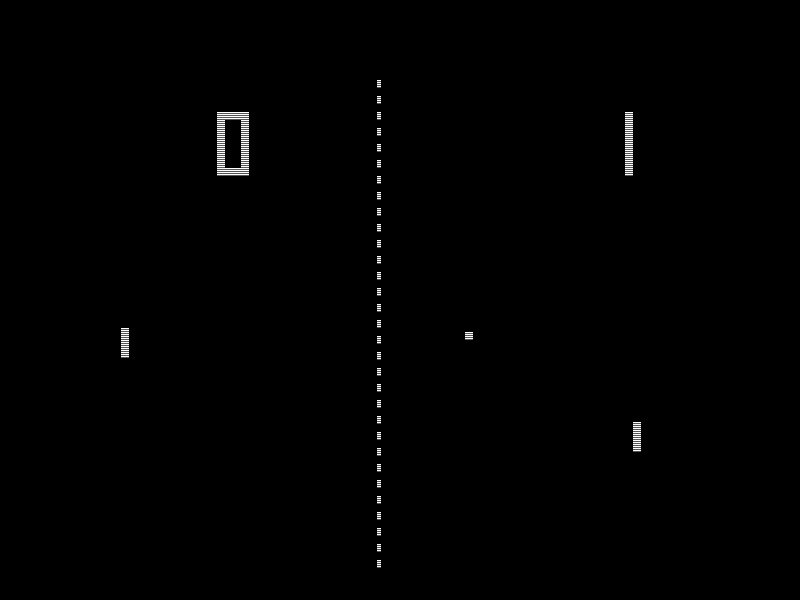
\includegraphics[height=0.2\paperheight]{pong-screenshot}
					\caption{\scriptsize\textbf{Pong} \copyright{1972} Atari\footnotemark{}}
				\end{figure}
				
			\column{0.7\textwidth}
			
				{\scriptsize
					\textbf{Objetivo}: fazer a bolinha cruzar o fundo da área do adversário\\
					\textbf{Condição de Término}: a bolinha ultrapassa a linha de fundo de um dos jogadores\\
					\textbf{Ações}: $1)$ mover o bastão para cima; $2)$ mover o bastão para baixo\\
					\textbf{Feedback}: $1)$ sinais sonoros do impacto da bolinha nos bastões, paredes e fundo de linha; $2)$ alteração do placar numérico; $3)$ movimentação dos bastões ao comando do jogador\\
					\textbf{Estéticas de experiência}: $1)$ curiosidade da interação com computadores (há época); $2)$ desafio e passatempo; $3)$ descoberta de habilidades (jogadas de efeitos); $4)$ interação social (``\textit{high score}''); $5)$ fantasia esportiva (tênis)
				}
			
		\end{columns}

	\end{block}	
	
	\footnotetext{\url{http://en.wikipedia.org/wiki/Pong}}
	
\end{frame}

% ---------------------------------------------------------------------------- %
\section{Atividade}
% ---------------------------------------------------------------------------- %

% ------------------------------
\begin{frame}
	\frametitle{\textbf{Desconstrução de jogos clássicos}}

	\vspace{-1.5em}

	\begin{center}
		Já em grupos, ``desconstrua'' os seguintes jogos:
	\end{center}
	
	\vspace{-1.5em}

	\begin{figure}
	    \centering

	    \begin{subfigure}[!h]{0.25\paperwidth}
	    	\centering
	    	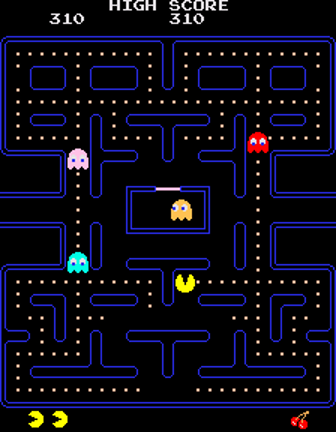
\includegraphics[height=0.22\paperheight]{pacman-screenshot}
	        \caption{\scriptsize\textbf{Pac-Man} \copyright{1980} Namco\footnotemark{}}
	    \end{subfigure}
	    ~
		\begin{subfigure}[!h]{0.25\paperwidth}
			\centering
	        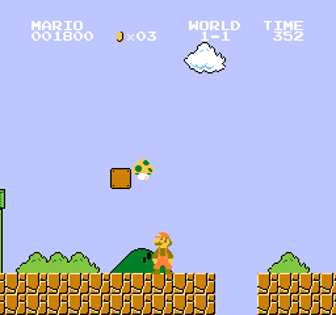
\includegraphics[height=0.2\paperheight]{supermario-screenshot}
	        \caption{\scriptsize\textbf{Super Mario Bros.} \copyright{1985} Nintendo\footnotemark{}}
	    \end{subfigure}
	   	~
	    \begin{subfigure}[!h]{0.25\paperwidth}
	    	\centering
	        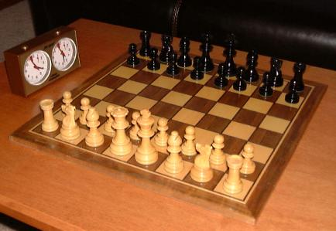
\includegraphics[height=0.2\paperheight]{chess-board}
	        \caption{\scriptsize\textbf{Xadrez}\footnotemark{}}
	    \end{subfigure}
	    \\[0.5em]
		\begin{subfigure}[!h]{0.35\paperwidth}
			\centering
	        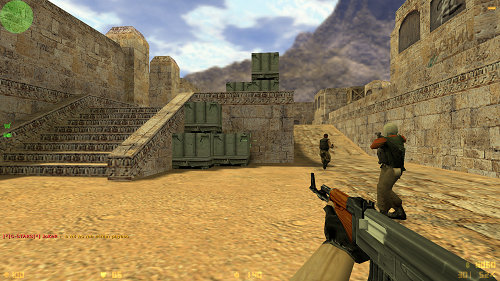
\includegraphics[height=0.2\paperheight]{cs-screenshot}
	        \caption{\scriptsize\textbf{Counter-Strike} \copyright{1999} Valve\footnotemark{}}
	    \end{subfigure}

    \end{figure}

	\footnotetext[4]{\url{http://www.arcade-museum.com/game_detail.php?game_id=10816}}
	\footnotetext[5]{\url{http://www.arcade-museum.com/game_detail.php?game_id=9913}}
	\footnotetext[6]{\url{http://pt.wikipedia.org/wiki/Xadrez}}
	\footnotetext{\url{http://en.wikipedia.org/wiki/Counter-Strike}}
    
\end{frame}

% ------------------------------------------
% References
% ------------------------------------------

\referencesbegin
\begin{frame}[plain, allowframebreaks]
	\frametitle{\textbf{References}}
	\bibliographystyle{abbrv}
	{\tiny \bibliography{bibliography}}
\end{frame}
\referencesend


\end{document}

